%-------------------------------------------------------------------------------
% CAPITOLO 16
%-------------------------------------------------------------------------------
\chapter{Lezione 16}
\label{capitolo_16}
\textit{Data: 26/04/2025}

\section{Ricerca del Filtro Ottimale}

\begin{equation} \label{eq:ch16_1}
n_{ext}^{opt}(\{i_k\}) = \sum_{k=1}^{N} \sum_{n_k=0}^{\infty} n_k \frac{ P(i_k, n_k)}{P(i_k)}
\end{equation}

Questo termine può essere riscritto come $\sum_{n_k=0}^\infty n_k P(n_k | i_k)$, cioè il valore atteso di $n_k$ data la corrente $i_k$.

\begin{equation} \label{eq:ch16_2}
n_{ext}^{opt}(\{i_k\}) = \sum_{k=1}^{N} \sum_{n_k=0}^{\infty} n_k P(n_k | i_k)
\end{equation}

Consideriamo il caso di bassa intensità luminosa, dove ogni fotorecettore $k$ assorbe al massimo un fotone ($n_k=0$ o $n_k=1$). Vogliamo calcolare $P(n_k|i_k)$.
Usiamo il teorema di Bayes:

\begin{equation} \label{eq:ch16_3}
P(n_k | i_k) = \frac{P(i_k | n_k) P(n_k)}{P(i_k)}
\end{equation}

Dove $P(n_k)$ è la probabilità a priori che il $k$-esimo fotorecettore assorba $n_k$ fotoni (dipende dall'intensità luminosa), e $P(i_k | n_k)$ è la probabilità di misurare la corrente $i_k$ dato che sono stati assorbiti $n_k$ fotoni (la nostra distribuzione Gaussiana del rumore). $P(i_k)$ è la probabilità marginale della corrente:

\begin{equation} \label{eq:ch16_4}
P(i_k) = \sum_{n'_k} P(i_k | n'_k) P(n'_k)
\end{equation}

Nel caso $n_k=0$ o $1$:

\begin{equation} \label{eq:ch16_5}
P(i_k) = P(i_k | n_k=0) P(n_k=0) + P(i_k | n_k=1) P(n_k=1)
\end{equation}

Assumiamo $P(i_k|n_k)$ Gaussiana con stessa varianza $\sigma^2$:

\begin{equation*} 
P(i_k | n_k=0) \approx \frac{1}{\sqrt{2\pi\sigma^2}} e^{-\frac{i_k^2}{2\sigma^2}}
\end{equation*}

\begin{equation*} 
P(i_k | n_k=1) \approx \frac{1}{\sqrt{2\pi\sigma^2}} e^{-\frac{(i_k - i_1)^2}{2\sigma^2}}
\end{equation*}

Calcoliamo $P(n_k=1 | i_k)$:

\begin{equation} \label{eq:ch16_6}
P(1 | i_k) = \frac{P(i_k | 1) P(1)}{P(i_k | 0) P(0) + P(i_k | 1) P(1)}
\end{equation}

Sostituendo le Gaussiane (omettendo il fattore $1/\sqrt{2\pi\sigma^2}$ che si cancella):

\begin{equation} \label{eq:ch16_7}
P(1 | i_k) = \frac{e^{-\frac{(i_k - i_1)^2}{2\sigma^2}} P(1)}{e^{-\frac{i_k^2}{2\sigma^2}} P(0) + e^{-\frac{(i_k - i_1)^2}{2\sigma^2}} P(1)}
\end{equation}

Dividendo numeratore e denominatore per $e^{-\frac{(i_k - i_1)^2}{2\sigma^2}} P(1)$:

\begin{equation} \label{eq:ch16_8}
P(1 | i_k) = \frac{1}{ 1 + \frac{P(0)}{P(1)} e^{ -\frac{i_k^2}{2\sigma^2} +\frac{(i_k - i_1)^2}{2\sigma^2} } } 
\end{equation}

Espandendo l'esponente: $-\frac{i_k^2}{2\sigma^2} + \frac{i_k^2 - 2i_k i_1 + i_1^2}{2\sigma^2} = \frac{-2i_k i_1 + i_1^2}{2\sigma^2} = -\frac{i_1}{\sigma^2} i_k + \frac{i_1^2}{2\sigma^2}$.

\begin{equation} \label{eq:ch16_9}
P(1 | i_k) = \frac{1}{1 + \frac{P(0)}{P(1)} e^{\frac{i_1^2}{2\sigma^2}} e^{-\frac{i_1}{\sigma^2} i_k}}
\end{equation}

Questa ha la forma di una funzione sigmoide:

\begin{equation} \label{eq:ch16_10}
P(1 | i_k) = \frac{1}{1 + e^{\theta - \beta i_k}}
\end{equation}

con

\begin{equation} \label{eq:ch16_11}
\theta = \ln\left( \frac{P(0)}{P(1)} e^{\frac{i_1^2}{2\sigma^2}} \right), \quad \beta = \frac{i_1}{\sigma^2}
\end{equation}

Questa funzione $P(1 | i_k)$ rappresenta la probabilità che un fotone sia stato assorbito, data la corrente $i_k$.

\begin{itemize}
    \item $P \approx 0$ per $i_k < \frac{\theta}{\beta}$
    \item $P \approx 1$ per $i_k < \frac{\theta}{\beta}$
\end{itemize}

\begin{figure}[h!]
\centering
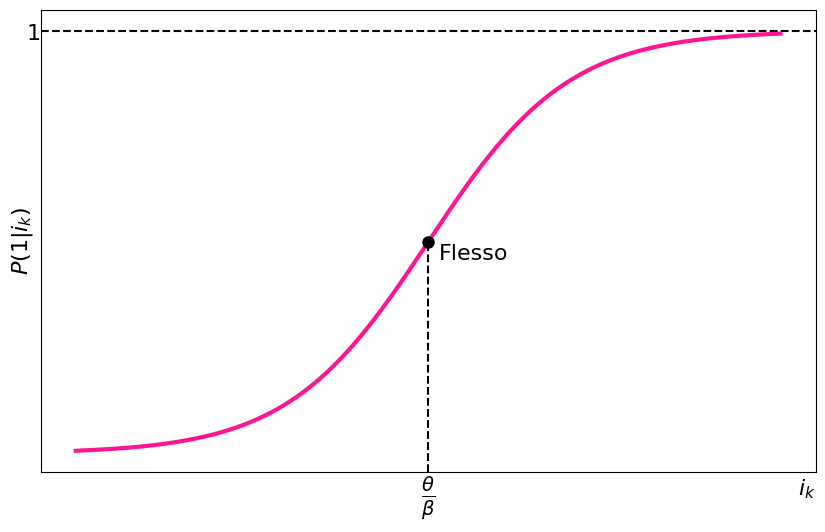
\includegraphics[width=0.6\textwidth]{pics/16_1.png} % INSERIRE QUI IL PERCORSO DEL GRAFICO
\caption{La probabilità che un fotone sia stato assorbito, data la corrente $i_k$.}
\label{fig:ch16_1}
\end{figure}

Quindi, il filtro ottimale diventa:

\begin{equation} \label{eq:ch16_12}
n_{ext}^{opt}(\{i_k\}) = \sum_{k=1}^{N} P(1 | i_k) = \sum_{k=1}^{N} \frac{1}{1 + e^{\theta_k - \beta i_k}}
\end{equation}

Questo risultato mostra che il filtro ottimale non è una semplice somma lineare delle correnti $i_k$. Ogni corrente $i_k$ viene pesata da un fattore non lineare $P(1|i_k)$ che dipende dalla corrente stessa. Le correnti che sono molto probabilmente dovute al rumore (cioè $i_k$ piccole in modulo, o comunque tali che $P(1|i_k) \approx 0$) contribuiscono poco alla somma, mentre quelle che sono molto probabilmente dovute all'assorbimento di un fotone ($P(1|i_k) \approx 1$) contribuiscono pienamente. Questo implementa un meccanismo di "noise gating" o filtraggio non lineare che migliora il rapporto segnale/rumore rispetto alla semplice somma lineare.

\begin{figure}[h!]
\centering
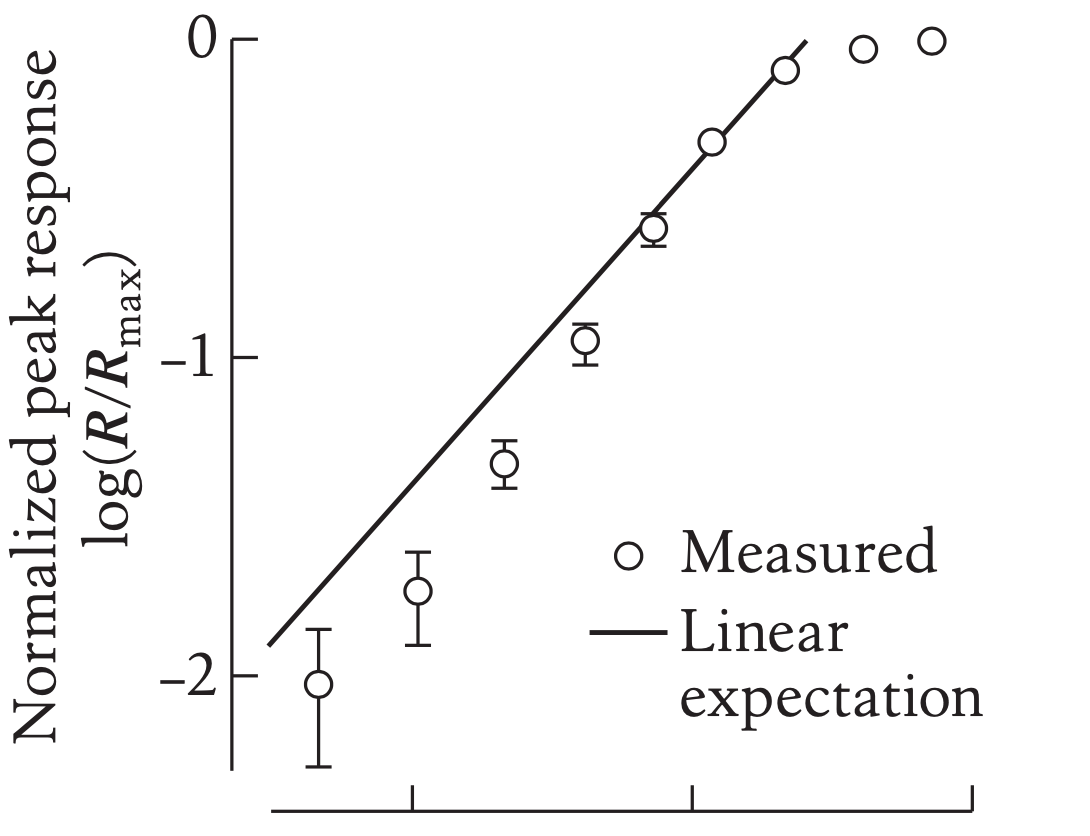
\includegraphics[width=0.6\textwidth]{pics/16_2.png} % INSERIRE QUI IL PERCORSO DEL GRAFICO
\caption{Ampiezze delle risposte di corrente (normalizzate al valore massimo) in funzione dell'intensità dello stimolo (in unità di $I_{1/2}$) (grafico log-log).}
\label{fig:ch16_2}
\end{figure}

L’andamento sperimentale è chiaramente non lineare.


\section{Modello di Ising}

Il modello di Ising rappresenta un sistema archetipico per lo studio dei comportamenti collettivi in fisica.
In questo modello, si considera un reticolo; su ogni sito reticolare è definita una variabile identificata come il momento magnetico individuale di spin dell'atomo situato sul sito. Tale variabile, denominata spin $s_i$, può assumere esclusivamente due valori:

\begin{itemize}
    \item $s_i = -1$: corrispondente a un momento magnetico di spin orientato verso il basso.
    \item $s_i = +1$: corrispondente a un momento magnetico di spin orientato verso l'alto.
\end{itemize}

\subsection*{Hamiltoniana del Modello di Ising}
L'energia del sistema, descritta dalla funzione Hamiltoniana $H$, è espressa come:

\begin{equation} \label{eq:ch16_13}
H = -\sum_{\langle i,j \rangle} J_{ij} s_i s_j - \sum_i h_i s_i 
\end{equation}

dove la somma $\langle i,j \rangle$ è ristretta alle coppie di primi vicini.

Il primo termine rappresenta l'interazione tra spin, o termine di allineamento.
$J_{ij}$ è una matrice che definisce quali coppie di spin interagiscono e l'intensità di tale interazione. Se $J_{ij} = 0$ per una specifica coppia di siti $i$ e $j$, gli spin localizzati su tali siti non interagiscono tra loro.
Si considera il caso in cui $J_{ij} = J > 0$ se i siti $i$ e $j$ sono primi vicini. Questa configurazione è nota come interazione a primi vicini. La definizione di "primi vicini" e il loro numero dipendono dalla geometria e dalla dimensionalità del reticolo.
Con $J > 0$, l'interazione è di tipo ferromagnetico e favorisce l'allineamento parallelo degli spin. Per minimizzare l'energia, il prodotto $s_i s_j$ deve essere positivo, il che implica che $s_i$ e $s_j$ abbiano lo stesso segno. Questo termine è detto di allineamento poiché la minimizzazione dell'energia si ottiene allineando gli spin.
Il secondo termine descrive l'interazione con un campo magnetico esterno $h_i$. Un campo magnetico esterno tende ad allineare gli spin parallelamente alla propria direzione.
In presenza di un campo magnetico, si manifestano due effetti competitivi: l'effetto del campo magnetico, che tende ad allineare ciascun spin a sé stesso, e l'effetto dell'interazione, per cui ciascun spin tende ad allinearsi con i propri vicini.
Questo modello è generalizzabile a sistemi non fisici, come quelli sociali, biologici o economici, in cui si osservano tendenze imitative (corrispondenti al termine di allineamento) e risposte a stimoli esterni (analoghi al campo magnetico).

\subsection*{Meccanica Statistica del Sistema}
Per l'analisi della meccanica statistica del sistema a una data temperatura, in equilibrio con un bagno termico, si impiega l'ensemble canonico. La quantità centrale da calcolare è la funzione di partizione $Z$.
Denotando con $S = \{s_1, s_2, \dots, s_N\}$ l'insieme di tutte le configurazioni di spin, la funzione di partizione è definita come:

\begin{equation} \label{eq:ch16_14}
Z = \sum_S e^{-\beta H(S)} 
\end{equation}

dove $\beta = 1/(k_B T)$, con $k_B$ costante di Boltzmann. La somma si estende a tutte le possibili configurazioni di spin $S$.
Ottenuta $Z$, si può determinare la misura di Boltzmann, ovvero la probabilità $P(S)$ associata a ciascuna configurazione di spin:

\begin{equation} \label{eq:ch16_15}
P(S) = \frac{1}{Z} e^{-\beta H(S)} 
\end{equation}

Utilizzando questa distribuzione di probabilità, è possibile calcolare il valore medio di qualsiasi osservabile, le sue fluttuazioni e altre grandezze termodinamiche.

\textbf{Energia Media:}
Il valore medio dell'energia $\langle E \rangle$ è dato da:

\begin{equation} \label{eq:ch16_16}
\langle E \rangle = \sum_S H(S) P(S) = \frac{1}{Z} \sum_S H(S) \; e^{-\beta H(S)} 
\end{equation}

Analogamente, per il valor medio del quadrato dell'energia, $\langle E^2 \rangle$:

\begin{equation} \label{eq:ch16_17}
\langle E^2 \rangle = \frac{1}{Z} \sum_S H(S)^2 e^{-\beta H(S)} 
\end{equation}

\textbf{Media di un'Osservabile Generica:}
Per una generica osservabile $O(S)$, il suo valore medio è:

\begin{equation} \label{eq:ch16_18}
\langle O \rangle = \sum_S O(S) P(S) = \frac{1}{Z} \sum_S O(S) e^{-\beta H(S)} 
\end{equation}

Una volta nota la funzione di partizione $Z$, è possibile derivare l'energia libera, l'entropia e altre funzioni di stato.

\subsection*{Analisi del Comportamento del Sistema}
Per semplicità, consideriamo inizialmente il caso senza campo esterno ($H_{ext} = 0$).

\begin{equation} \label{eq:ch16_19}
H = -J \sum_{\langle i,j \rangle} S_i S_j
\end{equation}

Questo modello descrive un comportamento puramente allelomimetico, ovvero di imitazione, molto comune nei sistemi biologici: ogni spin "vuole" essere simile ai suoi vicini.
Due fattori principali influenzano il sistema:
\begin{itemize}
    \item \textbf{a) L'ambiente (Temperatura):} L'ambiente introduce rumore nel sistema. In fisica statistica, questo rumore è modellato dalla temperatura $T$. Una temperatura elevata corrisponde a un grande rumore esterno, che tende a randomizzare l'orientamento degli spin, favorendo il disordine (aumento dell'entropia). Questo ambiente è detto bagno termico, ma può rappresentare qualsiasi fonte di rumore, come le perturbazioni ambientali per uno stormo di uccelli.
    \item \textbf{b) L'interazione:} L'interazione, rappresentata dal termine con $J$, si oppone al disordine e favorisce l'allineamento di tutti gli spin.
\end{itemize}

Analizziamo i casi estremi:

\subsubsection*{1) Caso a Temperatura Zero}
A $T=0$, il sistema cerca di raggiungere lo stato di energia minima. L'energia è minimizzata quando tutti gli spin sono allineati. Assumiamo che siano tutti orientati verso l'alto ($S_i = +1$ per ogni $i$).
L'energia di interazione si calcola sommando su tutte le coppie di primi vicini. Il numero di primi vicini di un sito è indicato con $z$ (es. su un reticolo quadrato, $z=4$).
L'energia minima del sistema sarà:

\begin{equation} \label{eq:ch16_20}
H_{min} = -J \frac{Nz}{2}
\end{equation}

Il fattore $1/2$ evita di contare due volte ogni coppia.
Esistono due stati che corrispondono a questa energia minima: quello con tutti gli spin up e quello con tutti gli spin down. Questo avviene perché l'Hamiltoniana possiede una simmetria di inversione degli spin: se invertiamo tutti gli spin di una qualsiasi configurazione, otteniamo una nuova configurazione con la stessa identica energia. Di conseguenza, anche lo stato di energia minima deve avere il suo "gemello" con spin invertiti. In questa condizione il sistema è perfettamente ordinato.

\subsubsection*{2) Caso a Temperatura Infinita}
Quando $T \rightarrow \infty$, $\beta \rightarrow 0$. Il fattore di Boltzmann $e^{-\beta H(S)}$ tende a 1 per qualsiasi configurazione.

\begin{equation} \label{eq:ch16_21}
P(S) = \frac{e^{-\beta H(S)}}{Z} \approx \frac{1}{Z}
\end{equation}

Ciò significa che tutte le configurazioni diventano equiprobabili. In questa situazione, il contributo dominante alle grandezze termodinamiche proviene dall'entropia. I macrostati più probabili sono quelli disordinati, poiché possono essere realizzati in un numero molto maggiore di microstati. Ad esempio, una configurazione con metà spin up e metà spin down ($K=N/2$) può essere ottenuta in $\binom{N}{K}$ modi, che è il valore massimo del coefficiente binomiale. Al contrario, gli stati perfettamente ordinati (tutti up o tutti down) sono unici.
In questo limite, l'interazione diventa trascurabile. L'energia fornita dal bagno termico è così alta che ogni spin fluttua in modo casuale e indipendente dagli altri.

\subsection*{Parametro d'Ordine e Transizioni di Fase}
Una quantità media di particolare rilevanza è il parametro d'ordine, che caratterizza lo stato macroscopico del sistema. Per il modello di Ising, il parametro d'ordine usuale è la magnetizzazione $M$.
La magnetizzazione totale (non normalizzata) è:

\begin{equation} \label{eq:ch16_22}
M = \sum_i \langle s_i \rangle 
\end{equation}

La magnetizzazione intensiva $m$ (magnetizzazione per spin) è:

\begin{equation} \label{eq:ch16_23}
m = \frac{1}{N} \sum_i \langle s_i \rangle 
\end{equation}

Si osservano due regimi distinti:
\begin{itemize}
    \item Ad alta temperatura ($T \to \infty$), i termini entropici sono dominanti. Il rumore termico induce fluttuazioni aleatorie e intense degli spin, prevalendo sull'effetto di allineamento. Il sistema non presenta un allineamento globale, risultando in $m \approx 0$. Questa fase è detta paramagnetica.
    \item A bassa temperatura ($T \to 0$), il termine energetico è preponderante e favorisce l'allineamento degli spin. Il sistema acquisisce una magnetizzazione non nulla, $m \neq 0$. Questa fase è detta ferromagnetica.
\end{itemize}

Variando la temperatura da valori elevati verso valori bassi, si identifica una temperatura critica $T_c$ alla quale il sistema transisce dalla fase paramagnetica a quella ferromagnetica. Tale transizione è una transizione di fase.

\begin{figure}[h!]
\centering
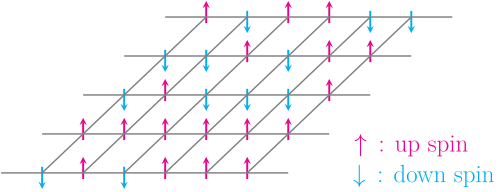
\includegraphics[width=0.6\textwidth]{pics/16_3.png} % INSERIRE QUI IL PERCORSO DEL GRAFICO DELLA MAGNETIZZAZIONE
\caption{Andamento della magnetizzazione $m$ in funzione della temperatura $T$.}
\label{fig:ch16_3}
\end{figure}

L'andamento di $m(T)$ mostra che:
\begin{itemize}
    \item $m=0$ per $T > T_c$
    \item $m \neq 0$ per $T < T_c$
\end{itemize}

Per $T < T_c$, il sistema manifesta un ordine ferromagnetico.

\vspace{0.5cm}
\noindent\fbox{%
    \parbox{\dimexpr\linewidth-2\fboxsep-2\fboxrule\relax}{%
        \textbf{!!}\\
        In assenza di un campo magnetico esterno ($h=0$), esistono due stati di equilibrio equivalenti: uno con tutti gli spin orientati verso l'alto ($m > 0$) e uno con tutti gli spin orientati verso il basso ($m < 0$).\\
        L'Hamiltoniana del sistema (con $h=0$) possiede una simmetria per inversione globale degli spin (cioè, $s_i \to -s_i$ per tutti gli $i$).\\
        Lo stato paramagnetico ($m=0$) è invariante rispetto a tale simmetria.\\
        Gli stati ferromagnetici ($m \neq 0$) rompono questa simmetria: l'inversione globale degli spin trasforma uno stato magnetizzato nell'altro, che è fisicamente distinto.\\
        Questo fenomeno è noto come rottura spontanea della simmetria. A livello macroscopico, il sistema può trovarsi in uno dei due stati di equilibrio distinti, ciascuno dei quali, singolarmente considerato, non possiede la piena simmetria dell'Hamiltoniana.
    }%
}
\vspace{0.5cm}

\subsection*{Approssimazione di Campo Medio (Mean Field)}
Risolvere esattamente il modello di Ising è un problema complesso. Per ottenere una comprensione qualitativa, si utilizza l'approssimazione di campo medio. L'idea è trasformare il sistema interagente in un sistema non interagente efficace.
Partiamo dall'Hamiltoniana completa con un campo esterno omogeneo $h$:

\begin{equation} \label{eq:ch16_24}
H = -J \sum_{\langle i,j \rangle} S_i S_j - h \sum_i S_i
\end{equation}

Il termine di interazione $\sum S_i S_j$ rende il problema difficile. L'approssimazione consiste nel riscrivere ogni spin $S_i$ come la somma del suo valore medio $m$ e di una fluttuazione $\delta S_i$:

\begin{equation} \label{eq:ch16_25}
S_i = \langle S_i \rangle + (S_i - \langle S_i \rangle) = m + \delta S_i
\end{equation}

Dato che il campo $h$ è omogeneo, il valore medio $\langle S_i \rangle$ è lo stesso per tutti i siti, $m_i = m$.
Sostituendo questa espressione nel termine di interazione:

\begin{equation} \label{eq:ch16_26}
S_i S_j = (m + \delta S_i)(m + \delta S_j) = m^2 + m(\delta S_i + \delta S_j) + \delta S_i \delta S_j
\end{equation}

Finora non abbiamo fatto alcuna approssimazione.
Il termine $\delta S_i \delta S_j$ accoppia le fluttuazioni degli spin sui siti $i$ e $j$. Questa è la parte più interessante e complessa, poiché descrive come gli spin tendano a fluttuare in modo coordinato.

\vspace{0.5cm}
\noindent\fbox{%
    \parbox{\dimexpr\linewidth-2\fboxsep-2\fboxrule\relax}{%
        L'approssimazione di campo medio consiste nel trascurare questo termine:
        \begin{equation} \label{eq:ch16_27}
        \delta S_i \delta S_j \approx 0
        \end{equation}
    }%
}
\vspace{0.5cm}

Fisicamente, questo equivale a dire che le fluttuazioni degli spin non sono correlate. Ogni spin non "vede" più le fluttuazioni istantanee dei suoi vicini, ma solo il loro effetto medio, rappresentato da $m$.
Con questa approssimazione, il termine di interazione nell'Hamiltoniana diventa:

\begin{equation} \label{eq:ch16_28}
\sum_{\langle i,j \rangle} S_i S_j \approx \frac{1}{2} \sum_{i \neq j} m_{ij} (m^2 + m\delta S_i + m\delta S_j)
\end{equation}

Dove $m_{ij}$ è la matrice di connettività (dice se due spin interagiscono).
Analizziamo i termini separatamente:

\textbf{Termine costante:}
\begin{equation} \label{eq:ch16_29}
\frac{1}{2} \sum_{i \neq j} m_{ij} m^2 = \frac{m^2}{2} \sum_{i} \sum_{j \neq i} m_{ij} = \frac{m^2}{2} \sum_{i} z = \frac{m^2 N z}{2}
\end{equation}

\textbf{Termini lineari nelle fluttuazioni:}
\begin{equation} \label{eq:ch16_30}
\frac{1}{2} \sum_{i \neq j} m_{ij} (m\delta S_i + m\delta S_j) = m \sum_{i \neq j} m_{ij} \delta S_j
\end{equation}

Ricordando che $\delta S_j = S_j - m$:

\begin{align}
m \sum_{i \neq j} m_{ij} (S_j - m) &= m \sum_j \left( \sum_{i \neq j} m_{ij} \right) S_j - m^2 \sum_{i \neq j} m_{ij} \nonumber \\  &= m z \sum_j S_j - m^2 N z \label{eq:ch16_31}
\end{align}

Mettendo insieme tutti i pezzi del termine di interazione approssimato:

\begin{equation} \label{eq:ch16_32}
\sum_{\langle i,j \rangle} m_{ij} S_i S_j \approx \frac{m^2 N z}{2} + m z \sum_j S_j - m^2 N z = - \frac{m^2 N z}{2} + m z \sum_j S_j
\end{equation}

Sostituendo questo risultato nell'Hamiltoniana, otteniamo l'Hamiltoniana di campo medio $H_{MF}$:

\begin{equation} \label{eq:ch16_33}
H_{MF} \approx -J \left( - \frac{m^2 N z}{2} + m z \sum_i S_i \right) - h \sum_i S_i
\end{equation}

Raggruppando i termini:

\begin{equation} \label{eq:ch16_34}
H_{MF} \approx \frac{J N z m^2}{2} - (h + J z m) \sum_i S_i
\end{equation}

Questa Hamiltoniana descrive un sistema di spin non interagenti. Il primo termine è una costante energetica, mentre il secondo mostra che ogni spin $S_i$ è soggetto a un campo efficace $h_{eff}$:

\begin{equation} \label{eq:ch16_35}
h_{eff} = h + J z m
\end{equation}

Questo campo efficace è la somma del campo esterno $h$ e del "campo molecolare" $Jzm$, che rappresenta l'influenza media di tutti i vicini sullo spin singolo.
Ora che il sistema è non interagente, possiamo calcolare facilmente la funzione di partizione.
La probabilità di una configurazione $S$ è:

\begin{equation} \label{eq:ch16_36}
P(S) = \frac{1}{Z} e^{-\beta H_{MF}(S)} = A \prod_i e^{\beta h_{eff} S_i} = \prod_i P(S_i)
\end{equation}

La probabilità si fattorizza, e la funzione di partizione totale $Z$ è il prodotto delle funzioni di partizione dei singoli spin, $Z = (Z_1)^N$. Calcoliamo $Z_1$ per un singolo spin, che ha Hamiltoniana $H_1 = -h_{eff}S_i$:

\begin{equation} \label{eq:ch16_37}
Z_1 = \sum_{S_i = \pm 1} e^{-\beta H_1(S_i)} = e^{\beta h_{eff}(+1)} + e^{\beta h_{eff}(-1)} = 2 \cosh(\beta h_{eff})
\end{equation}

\begin{equation} \label{eq:ch16_38}
Z_1 =  2 \cosh(\beta h_{eff})
\end{equation}

Infine, calcoliamo il valore medio di un singolo spin, che deve essere uguale alla magnetizzazione per sito $m$ che abbiamo introdotto all'inizio. Questa è la condizione di autocoerenza (self-consistency).

\begin{equation} \label{eq:ch16_39}
m  = \frac{1}{Z_1} \sum_{S_i = \pm 1} S_i e^{\beta h_{eff} S_i} = \frac{(+1)e^{\beta h_{eff}} + (-1)e^{-\beta h_{eff}}}{2 \cosh(\beta h_{eff})} = \frac{2 \sinh(\beta h_{eff})}{2 \cosh(\beta h_{eff})}
\end{equation}

\begin{equation} \label{eq:ch16_40}
m = \tanh(\beta h_{eff})
\end{equation}

Sostituendo l'espressione per $h_{eff}$, otteniamo l'equazione finale di autocoerenza per la magnetizzazione:

\begin{equation} \label{eq:ch16_41}
m = \tanh(\beta (h + Jzm))
\end{equation}

Questa equazione implicita lega la magnetizzazione $m$ a se stessa e ai parametri del sistema.
